\chapter{نمودارهای توالی تحلیل}


نمودارهای توالی مربوط به هریک از موارد کاربرد (با نام مشابه) به تفکیک زیرسیستم در این بخش ارائه می‌شود.

\newpage
\section{زیرسیستم کاربری}

\begin{figure}[ht!]
	\centering
	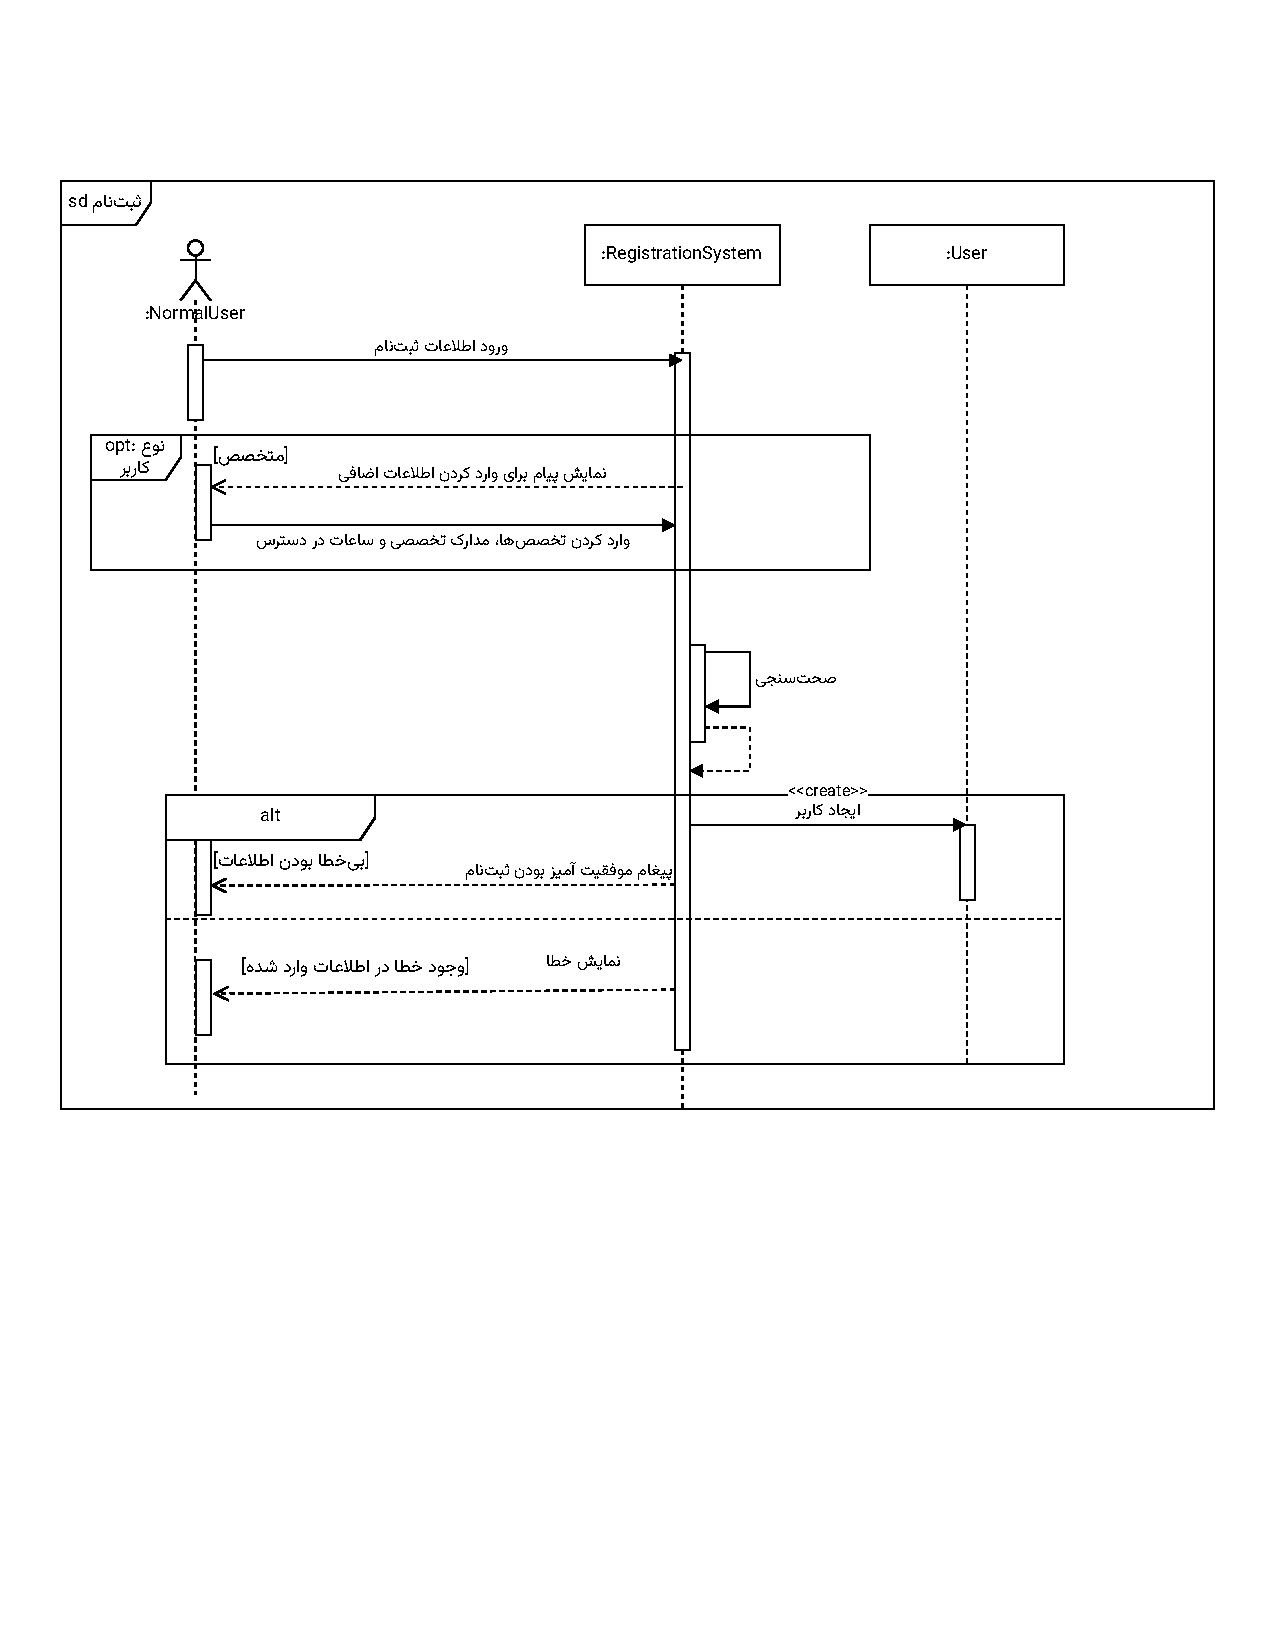
\includegraphics[scale=0.6, page=1]{figs/OOD-Sequence-1.pdf}
	\caption{نمودار توالی تحلیل: ثبت نام}
\end{figure}
\FloatBarrier
\newpage

\begin{figure}[ht!]
	\centering
	\includegraphics[scale=0.8, page=2]{figs/OOD-Sequence-1.pdf}
	\caption{نمودار توالی تحلیل: ورود}
\end{figure}
\FloatBarrier
\newpage

\begin{figure}[ht!]
	\centering
	\includegraphics[scale=0.8, page=3]{figs/OOD-Sequence-1.pdf}
	\caption{نمودار توالی تحلیل: خروج}
\end{figure}
\FloatBarrier
\newpage

\begin{figure}[ht!]
	\centering
	\includegraphics[scale=0.8, page=4]{figs/OOD-Sequence-1.pdf}
	\caption{نمودار توالی تحلیل: جست‌وجوی کاربران}
\end{figure}
\FloatBarrier
\newpage

\begin{figure}
	\centering
	\includegraphics[scale=0.8, page=5]{figs/OOD-Sequence-1.pdf}
	\caption{نمودار توالی تحلیل: مشاهده کاربران}
\end{figure}
\FloatBarrier
\newpage

\begin{figure}[ht!]
	\centering
	\includegraphics[scale=0.8, page=6]{figs/OOD-Sequence-1.pdf}
	\caption{نمودار توالی تحلیل: تایید متخصص}
\end{figure}
\FloatBarrier
\newpage

\begin{figure}[ht!]
	\centering
	\includegraphics[scale=0.8, page=7]{figs/OOD-Sequence-1.pdf}
	\caption{نمودار توالی تحلیل: اضافه کردن مدیر جدید}
\end{figure}
\FloatBarrier
\newpage

\begin{figure}[ht!]
	\centering
	\includegraphics[scale=0.8, page=8]{figs/OOD-Sequence-1.pdf}
	\caption{نمودار توالی تحلیل: ویرایش اطلاعات کاربری}
\end{figure}
\FloatBarrier
\newpage


\section{زیرسیستم خدمت‌دهی}


\begin{figure}[ht!]
	\centering
	\includegraphics[scale=0.6, page=9]{figs/OOD-Sequence-1.pdf}
	\caption{نمودار توالی تحلیل: فیلتر و مرتب‌سازی درخواست‌ها}
\end{figure}
\FloatBarrier
\newpage

\begin{figure}[ht!]
	\centering
	\includegraphics[scale=0.8, page=10]{figs/OOD-Sequence-1.pdf}
	\cccaption{نمودار توالی تحلیل: مشاهده درخواست‌ها}
\end{figure}
\FloatBarrier
\newpage

\begin{figure}[ht!]
	\centering
	\includegraphics[scale=0.8, page=11]{figs/OOD-Sequence-1.pdf}
	\cccaption{نمودار توالی تحلیل: مشاهده جزئیات درخواست}
\end{figure}
\FloatBarrier
\newpage

\begin{figure}[ht!]
	\centering
	\includegraphics[scale=0.8, page=2]{figs/OOD-Sequence-2.pdf}
	\cccaption{نمودار توالی تحلیل: انتخاب متخصص برای خدمت}
\end{figure}
\FloatBarrier
\newpage

\begin{figure}[ht!]
	\centering
	\includegraphics[scale=0.8, page=3]{figs/OOD-Sequence-2.pdf}
	\cccaption{نمودار توالی تحلیل: پذیرش درخواست مستقیم مشتری}
\end{figure}
\FloatBarrier
\newpage

\begin{figure}[ht!]
	\centering
	\includegraphics[scale=0.8, page=4]{figs/OOD-Sequence-2.pdf}
	\cccaption{نمودار توالی تحلیل: پذیرش درخواست دلخواه}
\end{figure}
\FloatBarrier
\newpage

\begin{figure}[ht!]
	\centering
	\includegraphics[scale=0.8, page=5]{figs/OOD-Sequence-2.pdf}
	\cccaption{نمودار توالی تحلیل: پذیرش متخصص}
\end{figure}
\FloatBarrier
\newpage

\begin{figure}[ht!]
	\centering
	\includegraphics[scale=0.8, page=6]{figs/OOD-Sequence-2.pdf}
	\cccaption{نمودار توالی تحلیل: لغو درخواست خدمت}
\end{figure}
\FloatBarrier
\newpage

\begin{figure}[ht!]
	\centering
	\includegraphics[scale=0.8, page=7]{figs/OOD-Sequence-2.pdf}
	\cccaption{نمودار توالی تحلیل: جست‌وجو و مشاهده متخصصین}
\end{figure}
\FloatBarrier
\newpage

\begin{figure}[ht!]
	\centering
	\includegraphics[scale=0.8, page=8]{figs/OOD-Sequence-2.pdf}
	\cccaption{نمودار توالی تحلیل: ثبت درخواست}
\end{figure}
\FloatBarrier
\newpage

\begin{figure}[ht!]
	\centering
	\includegraphics[scale=0.8, page=9]{figs/OOD-Sequence-2.pdf}
	\cccaption{نمودار توالی تحلیل: ثبت زمان انجام شدن خدمت}
\end{figure}
\FloatBarrier
\newpage

\begin{figure}[ht!]
	\centering
	\includegraphics[scale=0.8, page=10]{figs/OOD-Sequence-2.pdf}
	\cccaption{نمودار توالی تحلیل: ویرایش درخواست}
\end{figure}
\FloatBarrier
\newpage


\section{زیرسیستم بازخورد}


\begin{figure}[ht!]
	\centering
	\includegraphics[scale=0.6, page=11]{figs/OOD-Sequence-2.pdf}
	\cccaption{نمودار توالی تحلیل: ارزیابی خدمت دریافت شده}
\end{figure}
\FloatBarrier
\newpage

\begin{figure}[ht!]
	\centering
	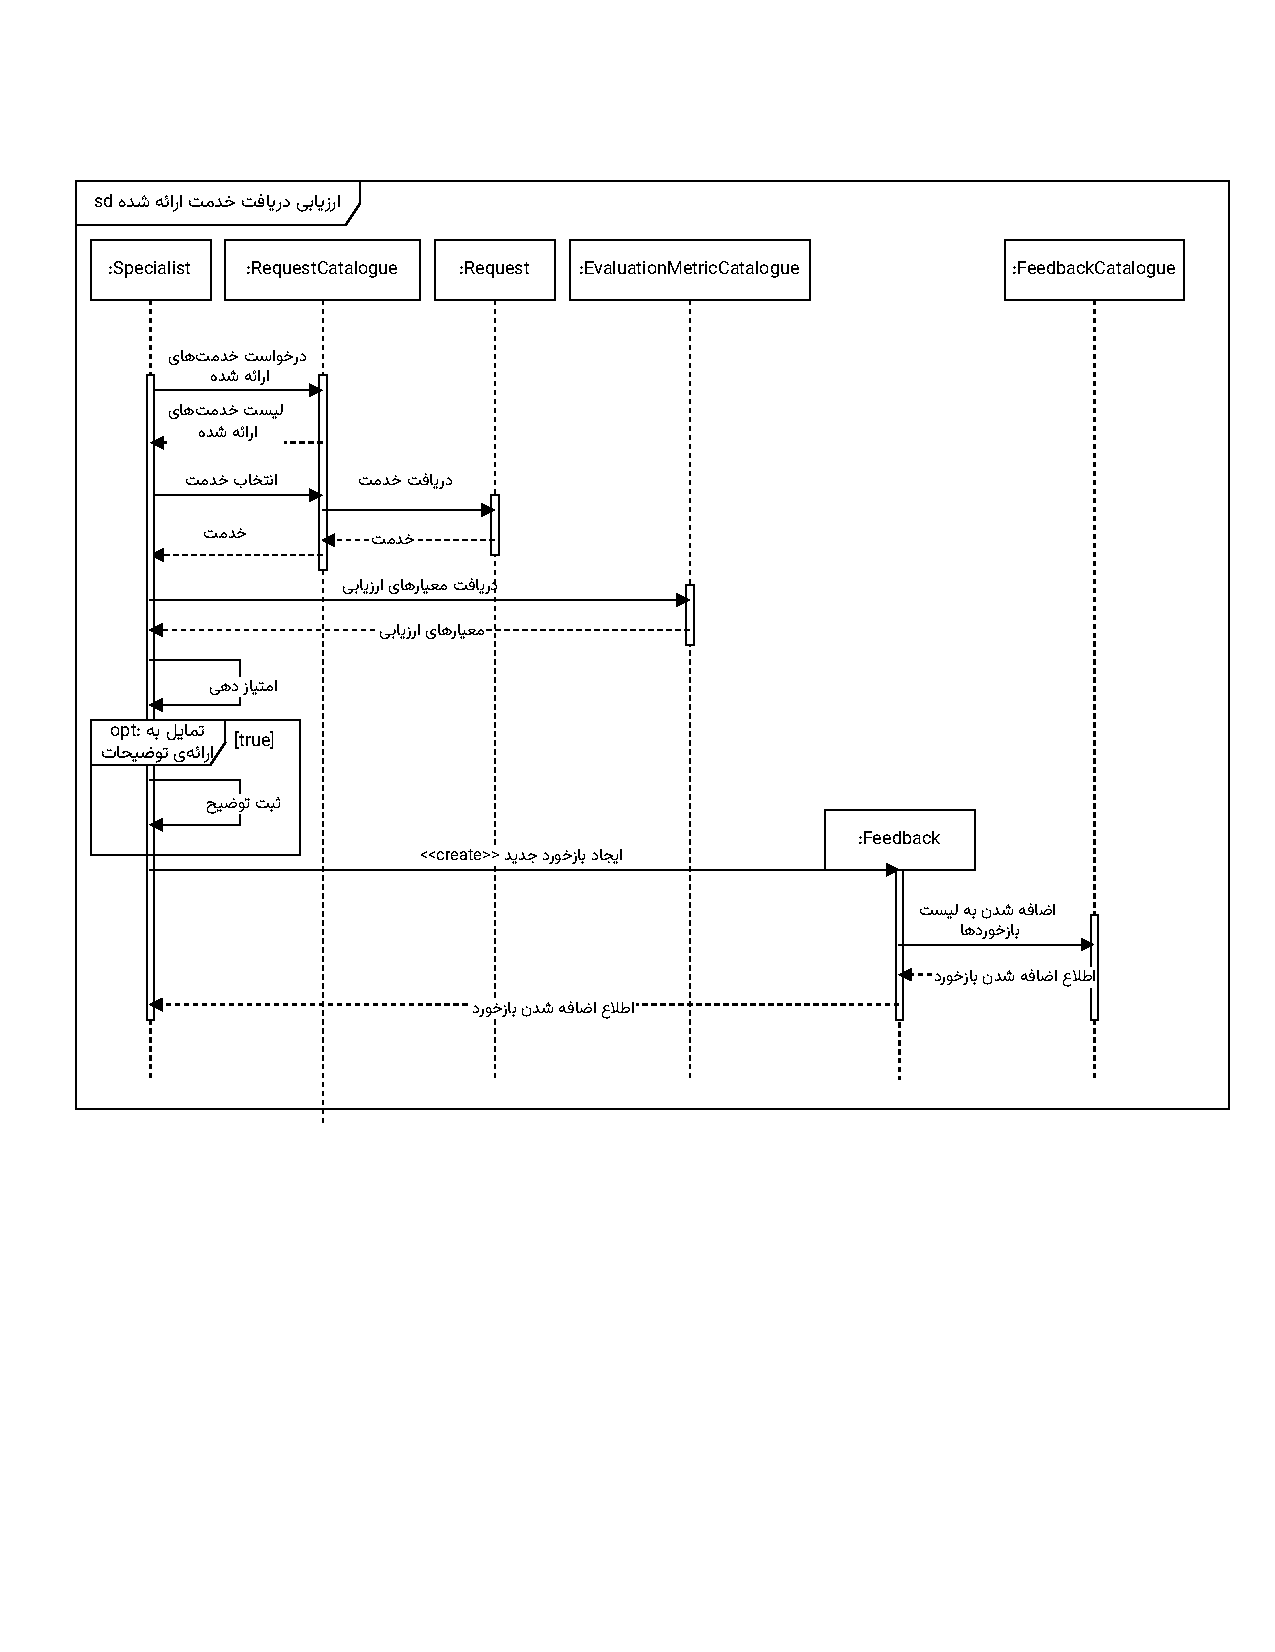
\includegraphics[scale=0.8, page=1]{figs/OOD-Sequence-3.pdf}
	\cccaption{نمودار توالی تحلیل: ارزیابی دریافت خدمت ارائه شده}
\end{figure}
\FloatBarrier
\newpage

\begin{figure}[ht!]
	\centering
	\includegraphics[scale=0.8, page=2]{figs/OOD-Sequence-3.pdf}
	\cccaption{نمودار توالی تحلیل: مشاهده لیست معیارهای ارزیابی}
\end{figure}
\FloatBarrier
\newpage

\begin{figure}[ht!]
	\centering
	\includegraphics[scale=0.8, page=3]{figs/OOD-Sequence-3.pdf}
	\cccaption{نمودار توالی تحلیل: اضافه کردن معیار ارزیابی}
\end{figure}
\FloatBarrier
\newpage

\begin{figure}[ht!]
	\centering
	\includegraphics[scale=0.8, page=4]{figs/OOD-Sequence-3.pdf}
	\cccaption{نمودار توالی تحلیل: ویرایش معیار ارزیابی}
\end{figure}
\FloatBarrier
\newpage

\begin{figure}[ht!]
	\centering
	\includegraphics[scale=0.8, page=5]{figs/OOD-Sequence-3.pdf}
	\cccaption{نمودار توالی تحلیل: حذف معیار ارزیابی}
\end{figure}
\FloatBarrier
\newpage

\begin{figure}[ht!]
	\centering
	\includegraphics[scale=0.8, page=6]{figs/OOD-Sequence-3.pdf}
	\cccaption{نمودار توالی تحلیل: ارسال پیشنهادات و انتقادات}
\end{figure}

\FloatBarrier
\newpage

\begin{figure}[ht!]
	\centering
	\includegraphics[scale=0.8, page=7]{figs/OOD-Sequence-3.pdf}
	\cccaption{نمودار توالی تحلیل: دریافت گزارش مشکلات فنی}
\end{figure}
\FloatBarrier
\newpage

\begin{figure}[ht!]
	\centering
	\includegraphics[scale=0.8, page=8]{figs/OOD-Sequence-3.pdf}
	\cccaption{نمودار توالی تحلیل: پاسخ به گزارش مشکل فنی}
\end{figure}
\FloatBarrier
\newpage

\section{زیرسیستم مدیریت}
\FloatBarrier
\begin{figure}[ht!]
	\centering
	\includegraphics[scale=0.8, page=9]{figs/OOD-Sequence-3.pdf}
	\cccaption{نمودار توالی تحلیل: اضافه کردن امتیاز مورد نیاز برای پذیرش درخواست}
\end{figure}
\FloatBarrier
\newpage


\begin{figure}[ht!]
	\centering
	\includegraphics[scale=0.8, page=10]{figs/OOD-Sequence-3.pdf}
	\cccaption{نمودار توالی تحلیل: ویرایش یا حذف امتیاز مورد نیاز برای پذیرش درخواست}
\end{figure}
\FloatBarrier
\newpage



\section{زیرسیستم چت}


\begin{figure}[ht!]
	\centering
	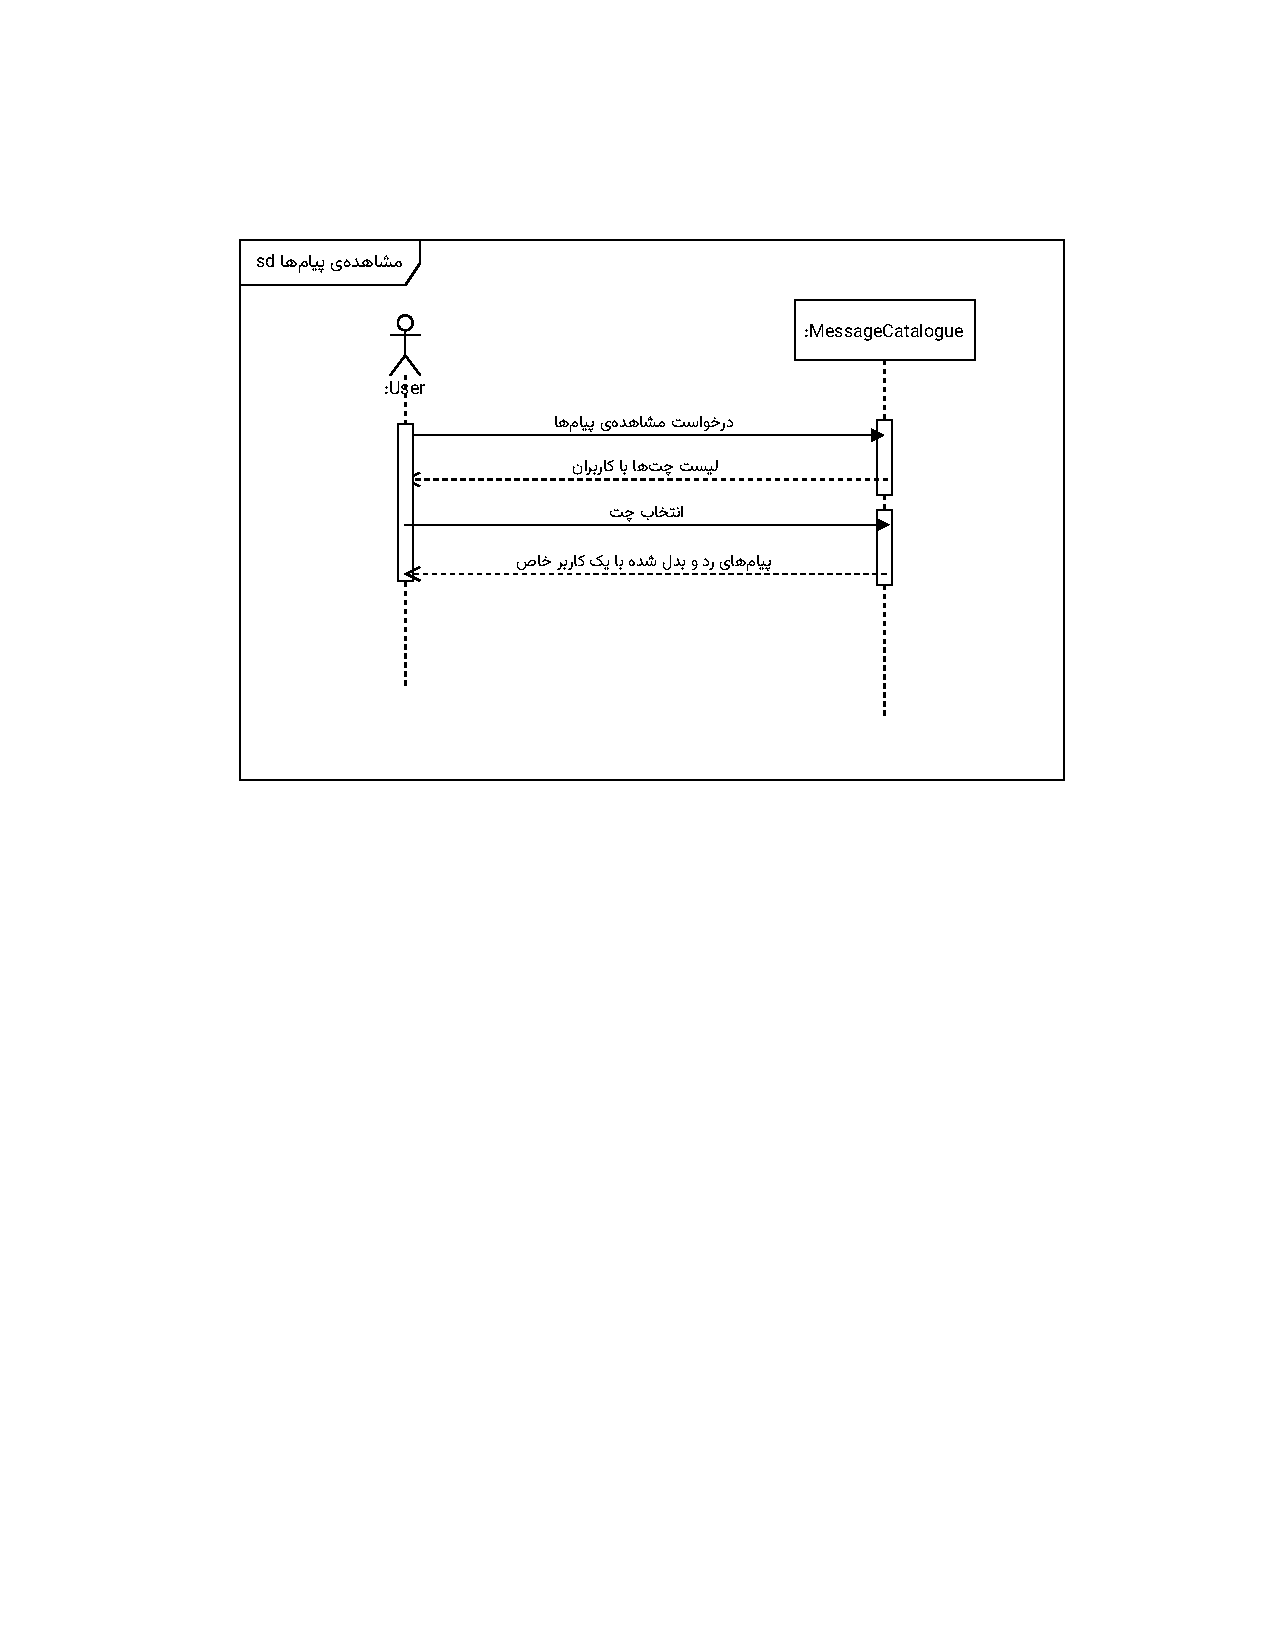
\includegraphics[scale=0.8, page=1]{figs/OOD-Sequence-chat.pdf}
	\cccaption{نمودار توالی تحلیل: مشاهده‌ی پیام‌ها}
\end{figure}
\FloatBarrier
\newpage

\begin{figure}[ht!]
	\centering
	\includegraphics[scale=0.8, page=2]{figs/OOD-Sequence-chat.pdf}
	\cccaption{نمودار توالی تحلیل: ارسال پیام}
\end{figure}
\FloatBarrier
\newpage



